La realización de este proyecto ha permitido alcanzar los objetivos que se planteaban al comienzo del mismo. En primer lugar se han investigado y evaluado diferentes formas y algoritmos para abordar la problemática inicial. Como consecuencia de ello se seleccionó la aproximación de Ellis al Vocoder de Fase. Posteriormente, trabajar en la implementación del prototipo ha permitido generar una versión parcialmente funcional del mismo en la placa proporcionada, en la que se han estudiado diferentes formas de lidiar con la problemática derivada del diseño, siendo necesario añadir modificaciones en el mismo a lo largo del periodo de trabajo. 

Es evidente que todo ello ha significado la consecución del objetivo último consistente en sintetizar y afianzar los conocimientos utilizados dentro de los diferentes ámbitos del proyecto: teoría de la señal y procesado de la misma, programación hardware, lenguaje VHDL, ciclo de desarrollo de producto y finalmente electrónica analógica.

Sin embargo, no ha sido posible completar la implementación del prototipo en el tiempo disponible, debido a que el ciclo de desarrollo de un aparato de estas características supera con creces la longitud del curso académico. Teniendo en cuenta la enorme cantidad de dificultades que han ido surgiendo a lo largo de este tiempo debido a lo novedoso del tema para mí y la dificultad para encontrar literatura útil para solucionarlos, me considero más que satisfecho con los resultados obtenidos.

En cuanto a características técnicas, el prototipo posee una latencia estimada en $30~ms$, \textbf{menor de lo esperado} en un principio. Además se han caracterizado los valores de consumo de recursos de la FPGA proporcionados por Vivado así como las medidas realizadas sobre el circuito analógico, que se encuentran en sus apartados correspondientes de la memoria. Como se ha comentado con anterioridad, estos resultados favorecen una \textbf{interpretación positivista} del proyecto, ya que se han superado las expectativas previas a la fase de montaje. Es evidente que \textbf{la razón para no utilizar FPGA en el mundo comercial y profesional no radica en las capacidades técnicas} de las mismas si no en otros factores como los económicos.

De cara a futuras ampliaciones sobre la materia, sería especialmente interesante culminar la realización del prototipo para permitir medir realmente su latencia y su calidad en el procesado. Una vez obtenidos estos datos, se podría mejorar el diseño optimizando las etapas existentes en el mismo, para lo que se aportan algunas ideas:

\begin{itemize}
\item Mejora del proceso de enventanado: estudio de como las diferentes ventanas y longitudes de las mismas (estrechamente relacionadas con la longitud de la transformada) afectan al rendimiento del conjunto.
\item Optimización de la etapa de transformación a frecuencia: es el proceso que más latencia puede provocar en el sistema en la zona de procesado. La mejora u optimización del mismo afecta en gran medida al rendimiento global. La manera en la que se introducen las diferentes tramas así como su modo de cálculo en cuanto a truncado, aproximaciones, desbordamientos y demás factores resultan fundamentales en la calidad del resultado.
\item Mejoras en la funcionalidad: añadir elementos comunes en el tratamiento de audio tales como control de volumen o panorámica estéreo acerca al diseño a un uso profesional real. Se han citado dos ejemplos, pero con la flexibilidad de la placa utilizada, existen infinidad de maneras facilitar su uso.
\item Implementación de algoritmos alternativos: evidentemente, tras comparar varios algoritmos sobre el papel, resultaría muy interesante diseñar las implementaciones de los mismos que permitiera la comparativa crítica entre ellos de manera práctica, ya que no existe casi ninguna sobre FPGA.
\end{itemize}

\begin{figure}[!h]
\begin{center}
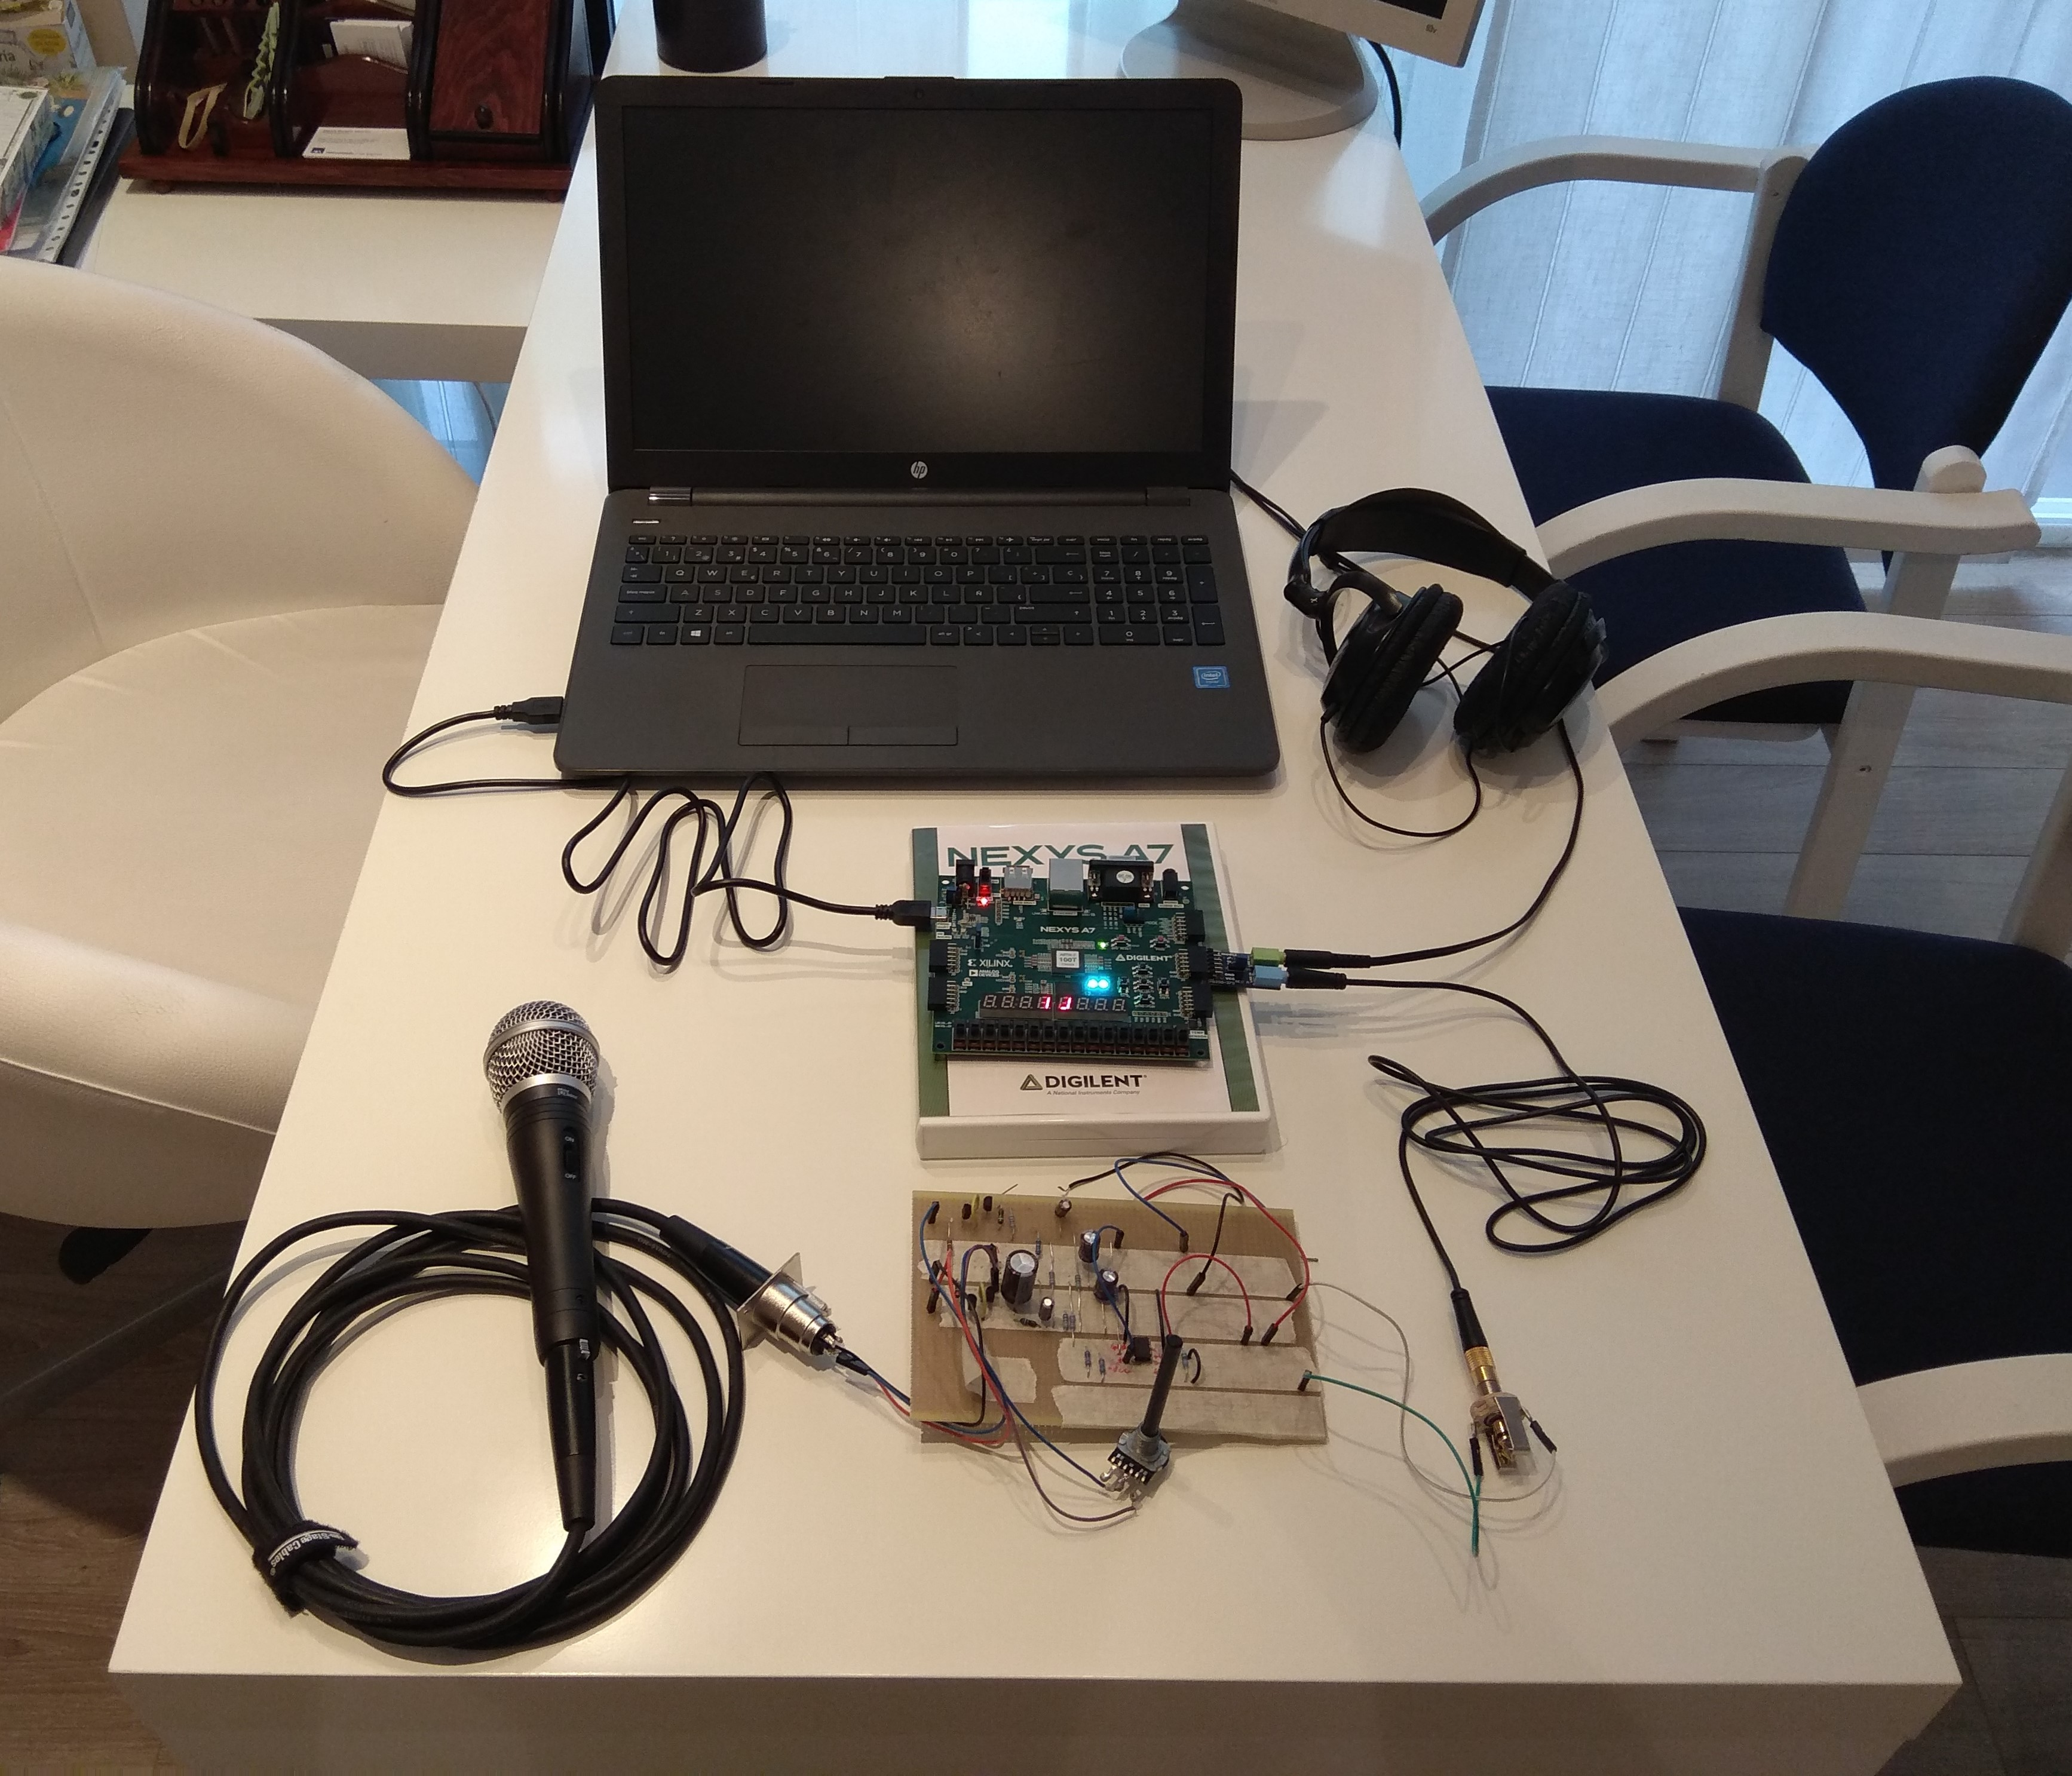
\includegraphics[width=14cm]{img/final.jpg}
%\caption{\label{fig:final}Conjunto final de los módulos desarrollados}
\end{center}
\end{figure}

